\documentclass[30pt, french]{tccv}
\usepackage[hmargin=0.2cm,vmargin=0cm]{geometry}
\usepackage{amsfonts} 								% for the \checkmark command 
\usepackage[framemethod=TikZ]{mdframed}						% For box around text
\usepackage[overlay,absolute]{textpos}						% For Textblock
\setlength{\TPHorizModule}{1cm}
\setlength{\TPVertModule}{1cm}
\usepackage{fontspec}								% For extended fonts
\usepackage{enumitem}								% For aptitudes enumeration 








\begin{document}
\begin{upshape}
\fontsize{10pt}{1.1em}\color{text}\selectfont



%%%%%%%%%%%%%%%%%%%%%%%%%%%%%%%%%%%%%%%%%%%%%%%%%%%%%%%%%%%%%%%%%%%%%%%%%%%%%%%%%%%%%%%%%%%%%%%%%%%%%%%%%%%%%%%%%%%%%%%%%%%%%%%%%%%%%%%%%%%%%%%%%%%%%%%%%%%%%%%%%%%%%%
%
%			0/ HEADER
%
%%%%%%%%%%%%%%%%%%%%%%%%%%%%%%%%%%%%%%%%%%%%%%%%%%%%%%%%%%%%%%%%%%%%%%%%%%%%%%%%%%%%%%%%%%%%%%%%%%%%%%%%%%%%%%%%%%%%%%%%%%%%%%%%%%%%%%%%%%%%%%%%%%%%%%%%%%%%%%%%%%%%%%




\begin{textblock}{6.5}(0.5,0.5)
\personal
    []
    {923 Route de la Roque sur Pernes 
    84800 Isle sur la Sorgue}
    {+33 6 79 59 85 38}
    {anne.martinez.sandoval@gmail.com}
\end{textblock}

\begin{textblock}{21}(2,1)
     \centering{\headerfirstnamestyle{Anne}   \headerlastnamestyle{Martinez}}
\end{textblock}

\begin{textblock}{21}(17.5,0.5)
		%%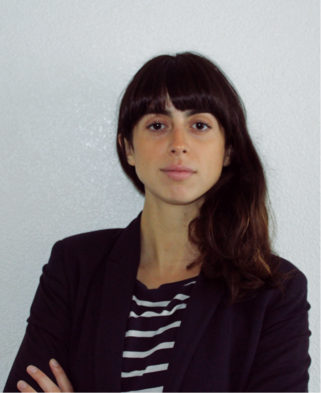
\includegraphics[width=3cm]{../Figure/Rocio3.png}
\end{textblock}  



\begin{textblock}{11}(7,2.3)
\begin{center}
\fontsize{10pt}{1.5em}\color{text}\bodyfontlight\upshape\selectfont

	{\fontsize{14pt}{5em}\scshape\bfseries \'Etudiante en Science Politique\\} 

	\vspace{5pt}
Œuvrer dans un environnement de travail au sein d’une institution internationale représentant de nouveaux et constants défis afin de développer mes capacités et acquérir de nouvelles connaissances. 
\end{center}
\end{textblock}  





%%%%%%%%%%%%%%%%%%%%%%%%%%%%%%%%%%%%%%%%%%%%%%%%%%%%%%%%%%%%%%%%%%%%%%%%%%%%%%%%%%%%%%%%%%%%%%%%%%%%%%%%%%%%%%%%%%%%%%%%%%%%%%%%%%%%%%%%%%%%%%%%%%%%%%%%%%%%%%%%%%%%%%
%
%			1/ EDUCATION
%
%%%%%%%%%%%%%%%%%%%%%%%%%%%%%%%%%%%%%%%%%%%%%%%%%%%%%%%%%%%%%%%%%%%%%%%%%%%%%%%%%%%%%%%%%%%%%%%%%%%%%%%%%%%%%%%%%%%%%%%%%%%%%%%%%%%%%%%%%%%%%%%%%%%%%%%%%%%%%%%%%%%%%%

\begin{education}
\item[Master 1 Science politique et Relations Internationales]{2016 -- 2017}
     {Lobatchevski Université, Russie}
     {     
     Année d’échange.\\
     \sloppy
     \tolerance 1000%
     Enseignement : Politique extérieure russe au Moyen-Orient ; 
     Théorie des relations internationales ; 
     Approche des organisations internationales ; 
     Histoire de la Russie ; 
     Langue russe.
     }
    
\item[Licence en Science Politique et Relations Internationales]{2013 -- 2014}
     {Centro de Investigación y Docencia Económicas (CIDE), Méxique}
     {Année d’échange.\\
     Enseignement : Politiques migratoires ; Amérique Latine : une étude régionale ; Information et communication ; Histoire du Mexique ; Relations Internationales.
     }

\item[Licence en Science Politique ]{2012 -- 2014}
     {Université Lumière Lyon 2, France}
     {Mention bien.\\
     Enseignement : Science Politique : approches et terrains ; Politiques comparée : les démocraties occidentales, Méthode des sciences sociales ; Partis et systèmes de partis ; La construction européenne. 
     }


\item[Baccalauréat Économique et Social]{2008 -- 2010}
     {Lycée Immaculée Conception, Carpentras, France}
     {Mention bien}
     
\vspace{-0.5cm}     
\section{Aptitudes}
\setlength{\parskip}{0pt}
\begin{itemize}[leftmargin=13pt]
  \setlength\itemsep{-3pt} 
  \fontsize{10pt}{1.1em}\color{text}\selectfont
  \cvitem[\checkmark]  Connaissances de la situation des Droits de l’Homme au Mexique
  \cvitem[\checkmark]  Analyse de discours officiels et comparaison avec les statistiques
  \cvitem[\checkmark]  Connaissances des politiques migratoires entre le Canada-Etats-Unis-Mexique
  \cvitem[\checkmark]  Rédaction et traduction de discours officiels
  \cvitem[\checkmark]  Organisation d’événements officiels
  \cvitem[\checkmark]  Traduction français-espagnol et anglais-espagnol
  \cvitem[\checkmark]  Maîtrise des réseau sociaux ainsi que des OS Windows et Mac. 
\end{itemize}



\end{education}


%%%%%%%%%%%%%%%%%%%%%%%%%%%%%%%%%%%%%%%%%%%%%%%%%%%%%%%%%%%%%%%%%%%%%%%%%%%%%%%%%%%%%%%%%%%%%%%%%%%%%%%%%%%%%%%%%%%%%%%%%%%%%%%%%%%%%%%%%%%%%%%%%%%%%%%%%%%%%%%%%%%%%%
%
%			2/ COMPETENCE
%
%%%%%%%%%%%%%%%%%%%%%%%%%%%%%%%%%%%%%%%%%%%%%%%%%%%%%%%%%%%%%%%%%%%%%%%%%%%%%%%%%%%%%%%%%%%%%%%%%%%%%%%%%%%%%%%%%%%%%%%%%%%%%%%%%%%%%%%%%%%%%%%%%%%%%%%%%%%%%%%%%%%%%%


\begin{competence}


\section{Compétences linguistiques}
\fontsize{15pt}{1.6em}\color{text}\bodyfontlight\upshape\selectfont %  increase most important
\begin{factlist}
\item{Français} {Langue maternelle}	
\item{Espagnol} {Bilingue}	
\item{Anglais} {Confirmé}	
\item{Russe} {Avancé}
\end{factlist}

\fontsize{10pt}{1.1em}\color{text}\bodyfontlight\upshape\selectfont % returnnormal 





%connaissance des outils bureautiques

\end{competence}




%%%%%%%%%%%%%%%%%%%%%%%%%%%%%%%%%%%%%%%%%%%%%%%%%%%%%%%%%%%%%%%%%%%%%%%%%%%%%%%%%%%%%%%%%%%%%%%%%%%%%%%%%%%%%%%%%%%%%%%%%%%%%%%%%%%%%%%%%%%%%%%%%%%%%%%%%%%%%%%%%%%%%%
%
%			3/ EXPERIENCE
%
%%%%%%%%%%%%%%%%%%%%%%%%%%%%%%%%%%%%%%%%%%%%%%%%%%%%%%%%%%%%%%%%%%%%%%%%%%%%%%%%%%%%%%%%%%%%%%%%%%%%%%%%%%%%%%%%%%%%%%%%%%%%%%%%%%%%%%%%%%%%%%%%%%%%%%%%%%%%%%%%%%%%%%


\begin{experience}

\vspace{0.5cm}
\item{\color{text} Octobre 2015 -- Mai 2016}
     {Université de Rennes 1}
     {Tutrice}
     \fontsize{10pt}{1.1em}\color{text}\bodyfontlight\upshape\selectfont
\mission{Contexte :} Tutrice au Bureau des Affaires Internationales de la faculté Droit/Science Politique \\
\sloppy
\tolerance 1000%
\mission{Missions :}      
    \setlength{\parskip}{-10pt}
    \begin{itemize}
      \cvitem[\checkmark] Participation au processus de sélection des étudiants rennais candidatant aux programmes Erasmus, Erasmus + et pro\-grammes d’échange hors Europe
      \cvitem[\checkmark] Traduction d’accords et communiqués officiels
      \cvitem[\checkmark] Accueil des étudiants étrangers et délégués d’uni\-ver\-sités par\-tenaires
    \end{itemize}     
\mission{Résultats :} Soutien du personnel du bureau dans certaines tâches administratives 



% COTE IVOIRE
\vspace{1.5cm}
\item{Avril 2014 -- Juin 2014}
     {Ambassade de Côte d’Ivoire à Mexico, Mexique}
     {Traducteur-Interprète}
     \fontsize{10pt}{1.1em}\color{text}\bodyfontlight\upshape\selectfont

\mission{Contexte : } Traducteur et interprète attachée au service économique et commercial de l’ambassade  \\
\mission{Missions :}      
    \setlength{\parskip}{-10pt}
    \begin{itemize}
      \cvitem[\checkmark] Participation à la « Feria de las Culturas Amigas 2014 » (la cinquième édition de la Feria des Cultures Amies), évènement de renommée internationale à Mexico DF qui accueille chaque année plus de 2 millions de personnes
      \cvitem[\checkmark] Accompagnement d’artistes ivoiriens venus spécialement pour exposer leurs dernières créations au Zócalo, l’artère principale de la capitale
    \end{itemize}     
\mission{Résultats :} Grande couverture médiatique et resserrement des liens d’amitié entre le Mexique et la Côte d’Ivoire


% MBELGIQUE
\vspace{1.5cm}
\item{Septembre 2014 -- Mars 2015}
     {Ambassade de Belgique à Mexico, Mexique}
     {Assistante}
     \fontsize{10pt}{1.1em}\color{text}\bodyfontlight\upshape\selectfont

\mission{Contexte : } Assistante attachée au service politique et culturel de l’ambassade \\
\mission{Missions :}      
    \setlength{\parskip}{-10pt}
    \begin{itemize}
      \cvitem[\checkmark] Analyse et suivi de l’information des contenus digitaux générée par les médias (officiels et non officiels) afin de faciliter l’identification de thèmes politiques et sociaux 
      \cvitem[\checkmark] Rédaction de synthèses sur l’actualité politique et sociale mexicaine
      \cvitem[\checkmark] Participation à des conférences et colloques organisés par le Ministère des Affaires Étrangères mexicain et par la Délégation Européenne
      %\cvitem[\checkmark] Participation à la « Feria de las Culturas Amigas 2014 » (la cinquième édition de la Feria des Cultures Amies), évènement de renommée internationale à Mexico DF qui accueille chaque année plus de 2 millions de personnes 
      %\cvitem[\checkmark] Accompagnement d’artistes ivoiriens venus spécialement pour exposer leurs dernières créations au Zócalo, l’artère principale de la capitale
    \end{itemize}     
\mission{Résultats :} Actualisation continue de la base de données et rapide transmission d’informations destinée au siège à Bruxelles 





\end{experience}





\end{upshape}
\end{document}
